\section{Experiments} \label{sec:experiments}


\subsection{Baseline Methods}

In this section we will go through the experiments performed in order to get
our baseline results. While many different features can be used when performing
\gls{NLP}, we chose the same features, as was used in \cite{US}, since they
span several several of the different linguistic layers. The linguistic
layers are different areas which all serve to describe a certain text. An
example this could be the character level layer, which as the name implies,
focuses on the individual characters used in a specific text. Other examples
of this, could the sentence, that focuses on the sentences of the text,
and the meta layer, that focuses on things such as publishing/delivery date,
and file format. The features available to pick from in this case are:

\begin{itemize}
    \item Word-N-grams,
    \item Character-N-grams,
    \item Word Frequencies (word-1-grams),
    \item \gls{POS}-tag-N-grams, and
    \item Special-Character-N-grams,
\end{itemize}

Where an N-gram describes the combinations of sequential elements of size n. In
the case where that element is characters, and n is 3, the string "hello" would
produce the character-3-grams "hel", "ell" and "llo". This also means that a
feature such as word frequencies can be considered word-1-grams.

For all of these experiments a Danish third party corpus, provided by
\texttt{NLTK}\footnote{\url{http://www.nltk.org/index.html}}, was used as the
basis for all the feature extraction, as was done in \cite{US} as well. This
corpus consists of 22,476 sentences, and 563,358 words.


\subsubsection{Extended Delta Method}

A large part of the experiments performed when applying the extended delta
method was parameter tuning. The extended delta method, does not do any
mitigation of noisy data or feature selection it self. Thus we would have
to do the feature selection ourselves. Not only that, but contrary to the
circumstances our previous paper \cite{US} was written in, we have more than
one text per author. As such, we don't need the opposing author approach any
more. When given a text $x$ and a proposed author $\alpha$, we pick out all
text written that author $T(\alpha)$, and a set different authored texts
$T_{diff}(\alpha)$ of same length. Using those sets, we create a \gls{KNN}
model, and apply it to $x$, returning 1 if $x \in T(\alpha)$ and zero otherwise.
Additionally we also apply the model to the negative case, where we pick text
randomly from the training-set, returning 1 if this new text is predicted as
being in $T_{diff}(\alpha)$ and 0 otherwise.

Thus we need to tune the K in \gls{KNN}, instead of the number of opposing
author that was used in \cite{US}

So the parameter selection consists of finding the best features, and the best
K.

Rather than finding the best features, using the somewhat random approach used
in our previous paper\cite{US}, we chose to do it more systematically this time
around. This however proved a greater task than anticipated. In order to find
the best set of feature, one would have to extract a very large set of features,
thousands in our case and determine the best combination of those features. A
task like that would take an incredible amount of computing power, and time.
Thus, we opted for a forward greedy selection approach.

We initially wanted to extract of large set of features, to perform our greedy
selection on. The corpus used had the following quantities of the different
features.

\begin{itemize}
    \item Word-2-grams - 188,472
    \item Character-2-grams - 2,178
    \item Word Frequencies - 27,535
    \item \gls{POS}-tag-2-grams - 219
    \item Special-character-2-grams - 524
\end{itemize}

These numbers are of course inflated due to the size of the corpus relative
to the actual text we are training on, and will continue to increase as we
increase the N in the N-grams. As a result of this, the frequency of each N-gram
decreases, and so does the impact each individual N-gram has. For this reason we
choose to only focus on a subset most frequent instances of each feature, which
also serves to limit the parameter search space.

Using the quantities listed above as inspiration, a feature set of 8,600
features was produced, containing

\begin{itemize}
    \item The 500 most frequent words,
    \item The 500 most frequent word-N-grams for $N \in \{2,3,4\}$,
    \item The 300 most frequent character-N-grams for $N \in \{2,...,10\}$,
    \item The 50 most frequent \gls{POS}-tag-N-grams for $N \in \{3,4\}$, and
    \item The 50 most frequent special-character-N-grams for $N \in \{2,3,4\}$.
\end{itemize}

The selection the quantities, bases on the number available in the corpus,
as listed earlier. As the for the N in the N-grams, \cite{aalykke2016} found
out that char-8-grams worked very well in his case, which is why N goes all
the way to 10 in the case of char-N-grams . Looking at the results
from \cite{US}, Word-N-grams mostly stopped occurring in texts when getting
to 4-grams, when looking at the result from \cite{US}. A similar thing
could be seen with the special-character-N-grams, where an increase in N,
wouldn't contribute anything. \gls{POS}-tag-N-grams were a really big burden
computationally, as such a reduction in possible N-values, had to be made.

These features were extracted from subset of the data-set described earlier
in section \ref{sec:data}. However it wasn't beholden to the same upper limit
character and unique character constraint, as the lack of memory isn't nearly
as severe as in the case of our \gls{NN}s. This data-set contained 14646
entries. The distribution of the texts over authors in this data-set isn't
very evenly spread. As such, we removed some data-entries, so $$\{\forall \alpha
\in \mathcal{A}: |T(\alpha)| = T_{min}\}$$ Where $T_{min}$ is the smallest amount
of texts associated with one author, in the case 4. Doing this decreased the
data-set entry quantity to 3748, with 937 different authors.

Having the features, we could then proceed with the greedy algorithm, which
works as follows. It starts out only using the most frequent of each of
the different features. Using this set it loops through each $\alpha \in
\mathcal{A}$ applying the extended delta methods, as described earlier in this
section. After each iteration the next, most frequent of each of the feature
is added to our active set of features, and then the extended delta method is
applied again. For each of these iteration, the best result is saved. If the
result doesn't improve for three iterations, or no more features are available,
the saved best result is returned. As each feature only has a certain of amount
of most frequent values, the greedy algorithm will reach a point where it want
to take grab the next most frequent feature, but it isn't available. In this
case, simple stop taking entries from that feature, but we keep taking from the
others. This greedy approach was applied using different configurations of the
N in KNN and distance metric, with $N \in {1,...,7}$, and the distance metric
being either Manhattan or Euclidean.

The results of the selection can be seen in figures \ref{fig:resultsMan} and 
\ref{fig:resultsEuc}. 

\begin{table}
    \centering
    \begin{tabular}{|c|c|c|}
    \hline
    KNN & Frequent Feature Count & Result          \\ \hline
    1   & 12                     & \textbf{0.7705} \\ \hline
    2   & 10                     & 0.6927          \\ \hline
    3   & 6                      & 0.6742          \\ \hline
    4   & 2                      & 0.6378          \\ \hline
    5   & 13                     & 0.6391          \\ \hline
    6   & 2                      & 0.6053          \\ \hline
    7   & 10                     & 0.5989          \\ \hline
    \end{tabular}
    \caption{Results of the forward greedy selection of the extended delta
        method using the Manhattan distance. The point where a single feature
        had no more entries to pick from, was never reached. As such Frequent
        Feature Count describes how many most frequent entries were picked out
        from each feature.}
    \label{fig:resultsMan}
\end{table}

\begin{table}[]
    \centering
    \begin{tabular}{|c|c|c|}
    \hline
    KNN & Frequent Feature Count & Result          \\ \hline
    1   & 10                     & \textbf{0.7772} \\ \hline
    2   & 13                     & 0.6990          \\ \hline
    3   & 3                      & 0.6791          \\ \hline
    4   & 4                      & 0.6499          \\ \hline
    5   & 2                      & 0.6288          \\ \hline
    6   & 2                      & 0.6065          \\ \hline
    7   & 2                      & 0.5959          \\ \hline
    \end{tabular}
    \caption{Results of the forward greedy selection of the extended delta
        method using the Euclidean distance. The point where a single feature
        had no more entries to pick from, was never reached. As such Frequent
        Feature Count describes how many most frequent entries were picked out
        from each feature.}
    \label{fig:resultsEuc}
\end{table}

As such, the best configuration is Euclidean distance, with the 10 most frequent
of the different features, is what we will be using on the test data.


\subsubsection{Author Specific SVM}

The author specific SVM is a authorship verification method that learns from
hand crafted features. Similar to the Extended Delta method we perform a feature
search in a large set of features to find the optimal features for the SVM. To
evaluate different feature sets and different hyperparameters we use the
algorithm shown in Figure \ref{fig:svm_evaluation_algorithm}. The algorithm
computes the average accuracy of the SVM via leave one out cross validation. For
each author it takes a set of texts written by that author and a set of texts of
similar size written by another author. Then it successively leaves out one of
the texts, train an SVM on the rest and then use that SVM to predict the class
of the text that was left out. The score is then the average accuracy of that
prediction.

\begin{figure}
    \begin{algorithm}[H]
        \KwData{$A$ set of authors, $F$ set of features, $C$ SVM hyperparameter,
            $\gamma$ SVM hyperparamter}
        Let $S = \emptyset$\;
        \For {$\alpha \in A$} {
            Let $T_k = T(\alpha)$\;
            Let $T_u = \{
                x_i\ |\ x_i \in \mathcal{U}\left(
                    \overline{T}(\alpha)
                \right), 1 \leq i \leq \left| T_k \right|
            \}$\;
            \label{line:draw_opposition}
            Let $F_k = \{ f(t, F)\ |\ t \in T_k\}$\;
            \label{line:feature_extract_1}
            Let $F_u = \{ f(t, F)\ |\ t \in T_u\}$\;
            \label{line:feature_extract_2}
            \For {$x \in F_k \cup F_u$} {
                Let $m = SVM(F_k \setminus x, F_u \setminus x, C, \gamma)$\;
                \uIf {$m(x) = a(x)$} {
                    Let $S = S \cup \{1\}$\;
                } \uElse {
                    Let $S = S \cup \{0\}$\;
                }
            }
        }
        \Return {$\mu(S)$}
        \caption{SVM evaluation}
    \end{algorithm}
    \caption{Algorithm to evaluate an SVM on a set of authors. The algorithm is
        given a set of authors $A$ to evaluate over, a set of features $F$ to
        use and the hyperparameters for the SVM. On Line
        \ref{line:draw_opposition} $\mathcal{U}$ denotes the uniform
        distribution and $T_u$ is a set of texts of the same size as $T_k$ where
        each text in the set is written by a different author than $\alpha$. On
        Line \ref{line:feature_extract_1} and Line \ref{line:feature_extract_2}
        $f$ denotes a function that computes the features $F$ of the text $t$.
        The algorithm computes the average accuracy of an SVM with the paramters
        given over all authors given.}
    \label{fig:svm_evaluation_algorithm}
\end{figure}

The search in a set of features $F$ are performed by starting with an
empty set of features $FC$. Then in each iteration we add a single
$f \in F$ to $FC$ and evaluate the SVM with the algorithm in Figure
\ref{fig:svm_evaluation_algorithm}. At the end we add only the single feature
that gives the best performance in the evaluation algorithm and repeat again
with the rest of the features. The feature set we search in are the same feature
set as the feature set used in the Extended Delta Method but without limiting
the number of texts per authors. The search are performed on only 100 random
authors in the set as it otherwise takes to long. The feature search is done
with fixed SVM hyperparameters which we tune afterwards. The hyperparameters
used during the search was $C = 100$ and $\gamma = 1000$. The feature search
surprisingly found only 6 features before no features could improve the
result further. The specific features were the character-2-gram " -", the
character-3-gram ", o", the character-4-gram ", at", the character-4-gram ",
so", the character-6-gram ", der " and the word-1-gram "giver". Most of the
features seem to look at what authors are writing immediately following commas.
We found the optimal hyper parameters for the SVM by splitting the dataset
in two parts. 80\% of the authors went in the training part and 20\% of the
authors went in the validation part. Then for each author in the training
dataset we varied $C \in (10^{-2}, 10^0, \dots, 10^{10})$ and $\gamma \in
(10^{-9}, 10^{-7}, \dots, 10^3)$ and evaluated an SVM using the algorithm in
Figure \ref{fig:svm_evaluation_algorithm} with the fixed feature set for each
combination of hyperparameters. After that we took a majority vote between the
authors chosen hyperparameters and chose that as the final hyperparameters. The
final hyperparameters were $C = 100$ and $\gamma = 1000$. We then evaluated our
chosen parameters both feature set and hyperparameters on the validation set. We
obtained an accuracy of 0.62980.

Since we were surprised that only 6 features were used we also tried to take a
feature set of the 50 most frequent features in each category. We again ran the
search for hyperparameters. This time we found that $C = 100$ and $\gamma = 10$
worked the best. We obtained an accuracy of 0.69552. So we were able to obtain a
higher accuracy by arbitrarily choosing the 50 most frequent features instead of
doing a structured search.

TODO: Try using all features.


\subsection{Siamese Neural Network - Iteration 1}

The network we used to try and solve the problem is shown in Figure
\ref{fig:network_1}. The Siamese part of the network is the Convolutional
Layer. We used 1000 filters of size 10. That means that 1000 different features
are supposed to be learned by the network and each feature can use a local
context of 10 characters to extract a feature. After the convolution we have a
max-over-time pooling layer. The layer takes the maximum value of each feature
such that we have 1000 features from each text. We then have a normal dense
neural network on top of that which are given the features of both texts. The
dense network is then supposed to learn how to compare the features from the two
texts. We have 1 dense hidden layer each with 500 neurons. At the end we have
a output layer with two outputs. The activation function for all layers except
the last one is the rectified linear unit and the activation function of the
last layer is the softmax function. The output of the network is a probability
distribution over the two classes.

The input to the network first goes through an embedding layer. The embedding
layer transforms integers into dense vectors of floating point numbers. The
embedding layer functions as a lookup table such that each integer is mapped
to the same dense vector. The embedding is trainable meaning that better
embeddings will be learned while the network is training.

\begin{figure}[htb]
    \centering
    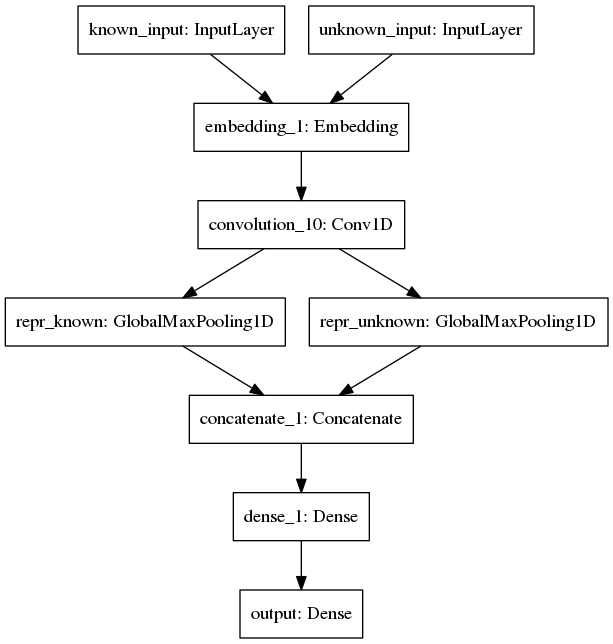
\includegraphics[width=0.6\textwidth]{./pictures/experiments/network1.png}
    \caption{Illustrate the structure of our first Siamese Neural Network
        Architecture.}
    \label{fig:network_1}
\end{figure}

The network obtained a validation accuracy of 0.68684. We have shown both the
training and validation accuracies in the different epochs in Figure
\ref{fig:network1_accuracies}. In that plot we can see that the network very
quickly overfits the training data and no longer learns anything general.

\begin{figure}[htb]
    \centering
    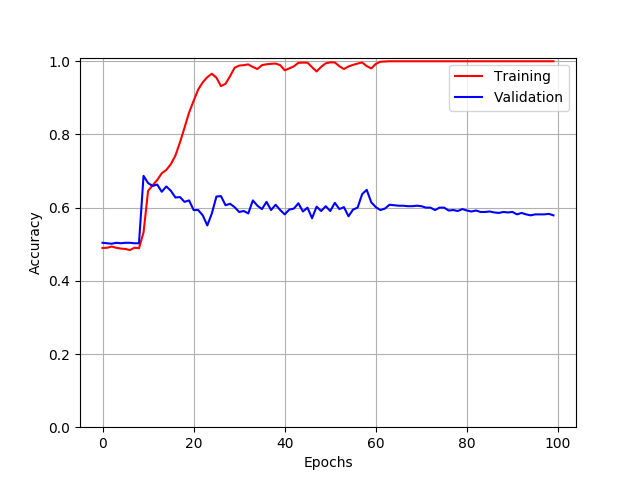
\includegraphics[width=0.5\textwidth]{./pictures/experiments/network_1_accuracies.png}
    \caption{Training and validation accuracies for the iteration 1 network in
        the different epochs of the networks execution.}
    \label{fig:network1_accuracies}
\end{figure}


\subsection{Siamese Neural Network - Iteration 2}

% TODO: Illustrate how dropout corresponds to training different subnetworks in
% each iteration.

In our last network we observed that the network after a few number of epochs
overfitted on the training dataset. The validation accuracy quickly began
stalling as the training accuracy went to 100\%. We therefore focused our
second network architecture on limiting overfitting. We added a dropout layer
before the output layer. The layer prevents overfitting by making sure that
the network cannot rely on the output of all neurons during training. This
unpredictability makes it harder for the network to learn specific quirks of
the training dataset since small quirks will only be picked up by a small
amount of neurons while larger trends will be represented by a larger set
of neurons. \cite{JMLR:v15:srivastava14a} investigated the use of dropout
layers in different problem settings. They found that dropout layers reduced
overfitting in all problems they looked at. In particular they found that
document classification which is similar to what we are doing were also
improved. The main drawback of a dropout layer is that it increase the run time
of training the networks (\cite{JMLR:v15:srivastava14a}).

In iteration 1 the function we used to merge features from the known and unknown
text together were a concatenation. If we let the extracted features of the
known text be $K_i$ and the extracted features of the unknown text be $U_i$ then
$K_0$ and $U_0$ correspond to the same feature extracted from the two texts. The
concatenation merge function would then produce,

\begin{equation}
    merge(K, U) \rightarrow \left(
        K_0, K_1, \dots, K_n, U_0, U_1, \dots, U_n
    \right)^T.
\end{equation}

That means that the neural network would have to figure out by itself that input
$0$ were related in particular to input $n + 1$. To save the network that task
we also replaced the merging function to the absolute difference of the feature
vectors. That means that our merge function became,

\begin{equation}
    merge(K, U) \rightarrow \left(
        (|K_0 - U_0|), (|K_1 - U_1|), \dots, (|K_n - U_n|)
    \right)^T.
\end{equation}

So the network no longer has to learn arbitrary indexes. Instead it can learn
which features is important for authorship verification and learn thresholds for
when each feature is important. With the new merging we will have a large number
whenever the two features are far apart and a small number whenever they are
close to each other.

We changed the convolutional filters we used from 1000 convolutional filters of
size 10 to 500 convolutional filters of size 4 and 500 convolutional filters of
size 8. The idea was that the filters could learn different features where some
of the features would consist of a large number of characters and other of the
features would consist of a small number of characters. The architecture of our
network from iteration 2 is shown in Figure \ref{fig:network_2}.

\begin{figure}
    \centering
    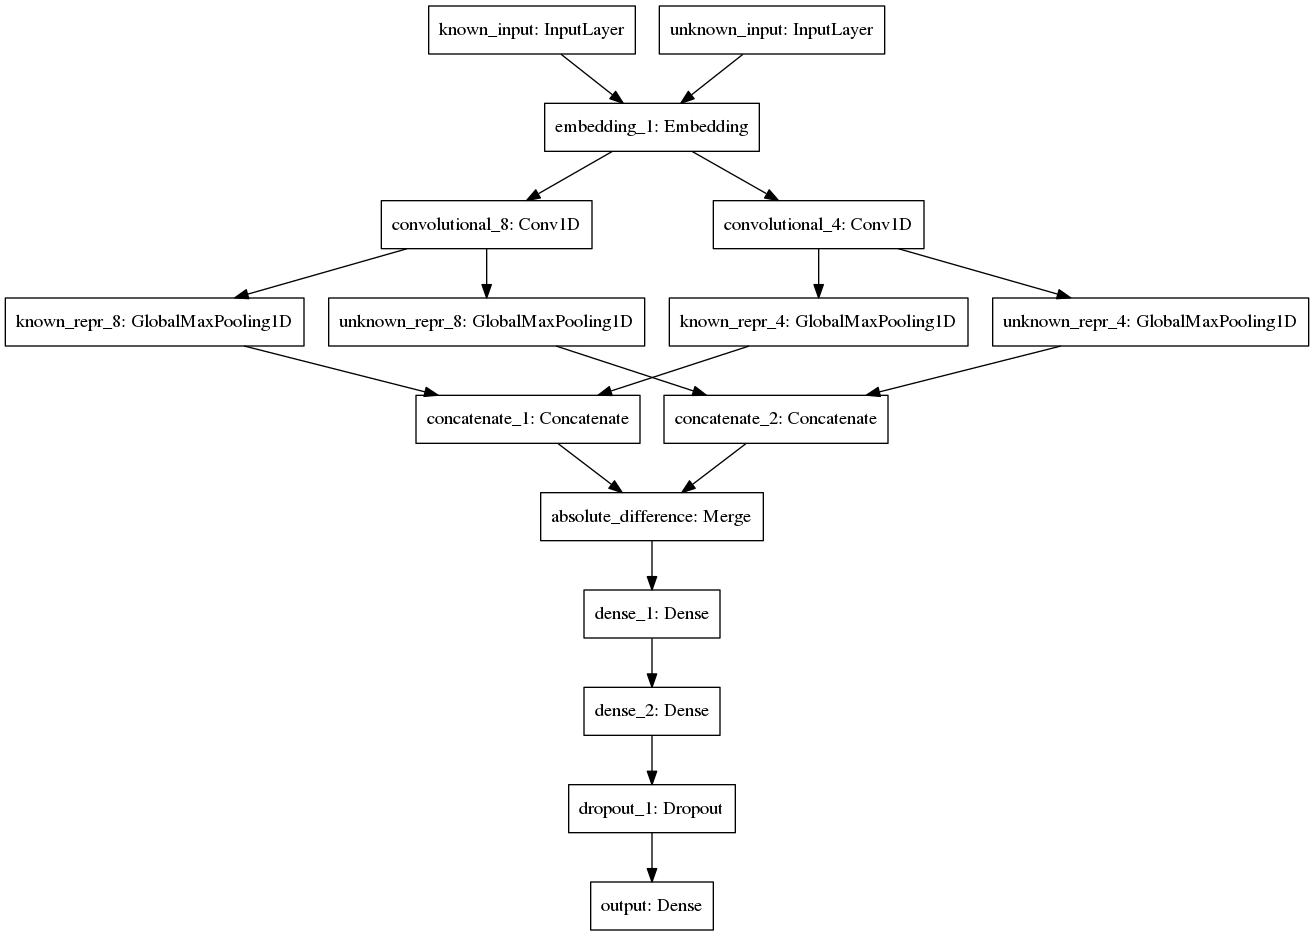
\includegraphics[width=\textwidth]{./pictures/experiments/network2.png}
    \caption{Illustrate the structure of our second Siamese Neural Network
        Architecture.}
    \label{fig:network_2}
\end{figure}

We also added more dense layers to the model. A plot of the
training and validation accuracies per epoch can be seen in Figure
\ref{fig:network2_accuracies}.

\begin{figure}
    \centering
    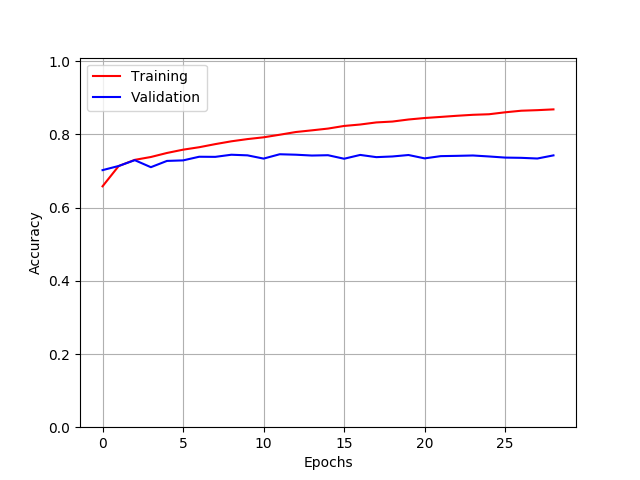
\includegraphics[width=0.5\textwidth]{./pictures/experiments/network_2_accuracies.png}
    \caption{Shows the training and validation accuracies on the second
        network.}
    \label{fig:network2_accuracies}
\end{figure}

The maximum validation accuracy obtained were 0.74464 in epoch 12.


\subsection{Siamese Neural Network - Iteration 3}

In iteration 2 we observed that the network seemed to learn everything in the
first epoch and didn't improve much after that. We also observed that the
accuracy improved compared to the first network. We therefore wanted to try a
larger network which would be able to hopefully learn more and obtain a higher
accuracy than our first two networks.

We both tried adding more convolutions and adding more dense layers. Our third
network use 700 convolutions of size 8 (currently drawn confusingly) and 500
convolutions of size 4. The network then contains 4 dense layers all with 500
hidden neurons with \gls{ReLu} activation function. Then a dropout layer with
30\% dropout and finally the output layer with 2 neurons and a softmax
activation function. The function we use to combine the features from the two
texts are still the absolute difference as that seemed to work fine for the
previous network. We have shown the structure of the third network in Figure
\ref{fig:network3}.

\begin{figure}
    \centering
    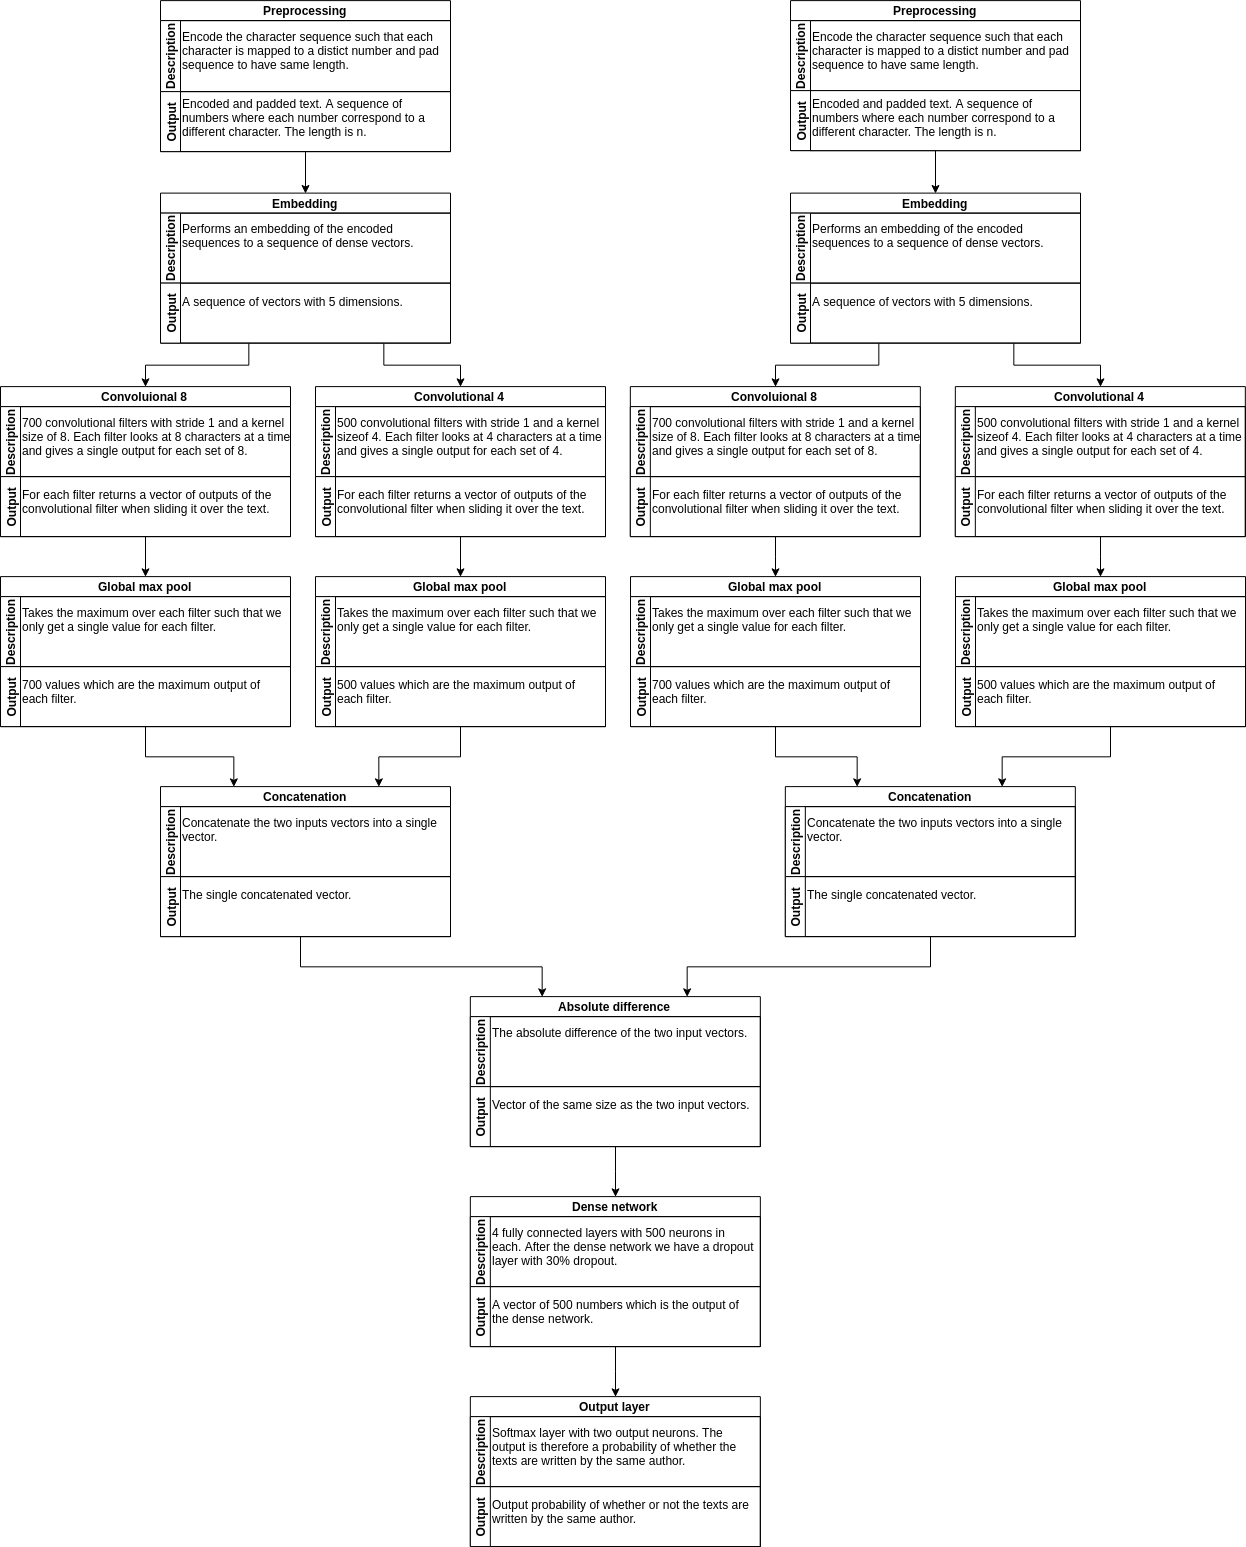
\includegraphics[width=\textwidth]{./pictures/experiments/network3.png}
    \caption{Illustrate the structure of our third Siamese Neural Network.
        Weights are shared by the embedding layers and the convolutional
        layers.}
    \label{fig:network3}
\end{figure}

Our third network were able to obtain an accuracy of 0.83612. We have shown the
training and validation accuracies in Figure \ref{fig:network_3_accuracies}. We
can see that the network quickly improve to about 80\% accuracy and after that
not much happens.

\begin{figure}
    \centering
    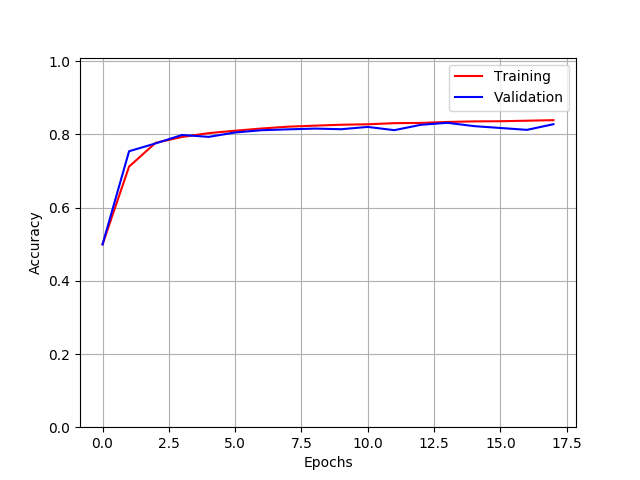
\includegraphics[width=0.5\textwidth]{./pictures/experiments/network_3_accuracies.png}
    \caption{Shows the training and validation accuracies over the epochs of
        training on the third network.}
    \label{fig:network_3_accuracies}
\end{figure}

To get an idea of which features the network were looking at we looked at the
output of the convolutional layers. After the convolutional layers we have a
max-over-time pool so we know that higher values are important. We could then
take a text, feed it to the network, find the index of the maximum output of
the convolutional layers and then show the text snipped (char-N-gram) that
produced that high value. We then did that for all the texts in the dataset. The
first filter in the network for example yielded many short strings ending with 3
newlines. Some examples of these are,

\begin{lstlisting}[gobble=4]
    'adsen\n\n\n'
    'ndsen\n\n\n'
    'umeer\n\n\n'
    'endte\n\n\n'
    'ingen\n\n\n'
    'ehren\n\n\n'
    'elsen\n\n\n'
    'ommer\n\n\n'
    'Ruter\n\n\n'
    'ummer\n\n\n'
    'ersen\n\n\n'
    'ansen\n\n\n'
    'heden\n\n\n'
    'ensen\n\n\n'
    'arsen\n\n\n'
    'orten\n\n\n'
    'ulsen\n\n\n'
    'orgen\n\n\n'
\end{lstlisting}

Many of those short string looks like the ending of common Danish
names followed by three newlines. Here are some examples of the
names taken from a list of the 100 most frequent surnames in Denmark
\footnote{http://www.mydanishroots.com/surnames-meaning-and-origin/the-100-most-
common-surnames-in-denmark.html},

\begin{description}
    \item[adsen:] Madsen.
    \item[ndsen:] Svendsen, Frandsen.
    \item[elsen:] Nielsen, Mikkelsen.
    \item[ersen:] Pedersen, Andersen, Petersen, Iversen, Jespersen.
    \item[ansen:] Hansen, Christiansen, Johansen, Kristiansen.
    \item[ensen:] Jensen, Christensen, S\o rensen, J\o rgensen, Kristensen,
        Mortensen, Mogensen.
    \item[arsen:] Larsen.
    \item[ulsen:] Poulsen.
\end{description}

The network therefore seems to have learned that a name followed by whitespace
are an important feature when determining the authorship of a text. Clearly when
a student buy an assignment from a ghost writer the text will contain the
students own name. Therefore these features are counter productive since the
network learns that as a result of how we have created the training dataset
where each text has the correct authors name in it.


\subsection{Siamese Neural Network - Iteration 4}

In this iteration we trained the third network again but now using a dataset
where names were substituted by empty strings. We wanted to see how well the
network would perform when it was not able to use peoples names as a feature.
A graph of the training and validation accuracies can be seen in Figure
\ref{fig:network_4_accuracies}. The best validation result we found was in epoch
20 with an accuracy of 0.80531. That means that we lost about 3\% accuracy now
that we can no longer look at peoples names.

\begin{figure}
    \centering
    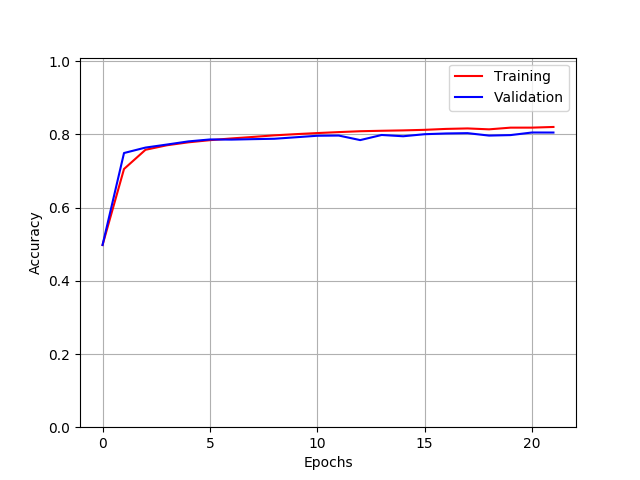
\includegraphics[width=0.5\textwidth]{./pictures/experiments/network_4_accuracies.png}
    \caption{Shows the training and validation accuracies over the epochs of
        training on the fourth iteration of the network.}
    \label{fig:network_4_accuracies}
\end{figure}

We wanted to verify whether or not the network still looked at the names of the
authors. It is not possible for us to look at all 1200 filters but we looked
at a couple and did not find any that looked like they were looking at names.
However we did find that the network now seems to be looking at which class
the student is in. The classes in Danish schools are typically written as 1.p,
1.q, 2.p, 2,q, etc. and we found that one of the convolutional 4 filters were
looking at character sequences such as those. We have generated a couple of
tables that shows what the network is now looking at. We generated the tables by
taking the first 50 texts from the dataset and extracting the maximum value of a
particular filter from each text. That gives a single string of the convolution
size from each text and a number which is higher the more important that string
is. We then sorted the extractions by the importance score. The result of a
couple of the filters are shown in Figures \ref{fig:features_convolution_8_1},
\ref{fig:features_convolution_8_5}, \ref{fig:features_convolution_8_100} and
\ref{fig:features_convolution_4_100}. The first figure looks at whether or not
authors use the phrase "s\aa\ at" (such that). Inexperienced Danish writers will
often use the phrase which is considered grammatically incorrect in most Danish
sentences. Therefore the network seems to have learned that some writers use
"s\aa\ at" while others don't and that it is an important phrase when verifying
authorship. The second figure seems to look at whether or not an authors uses
the phrase "meget" (most). Some authors apparently often describe things using
"meget" while others do not. The third figure shows that the network looks at
which authors use the phrase "at de" or "at der" ("that they" or "that there").
The fourth filter is the one that seems to look at which class a student is in.
In our constructed dataset the class of a student will always be a good feature
since we don't have any actual ghost writers. However a ghost writer would write
the correct class of the student on their submission. Therefore we don't want
the network to learn that particular feature.

\begin{table}
    \centering
    \textbf{Convolutional Filter 1 of Size 8}\par\medskip
    \begin{tabular}{c|cc}
        & \textbf{Filter Max String} & \textbf{Filter Max Value} \\ \hline
        \textbf{Text 13}  & \verb{', så at '{  & 44.41869 \\
        \textbf{Text 49}  & \verb{'2 se at '{  & 42.97375 \\
        \textbf{Text 29}  & \verb{'omas at '{  & 42.86139 \\
        \textbf{Text 21}  & \verb{'n nå at '{  & 42.27350 \\
        \textbf{Text 48}  & \verb{'r så at '{  & 41.95458 \\
        \textbf{Text 20}  & \verb{', nu et '{  & 41.92461 \\
        \textbf{Text 26}  & \verb{'t se at '{  & 41.03944 \\
        \textbf{Text 17}  & \verb{'m af at '{  & 40.85154 \\
        \textbf{Text 10}  & \verb{'mene at '{  & 40.75563 \\
        \textbf{Text 16}  & \verb{'mene at '{  & 40.75563 \\
        \textbf{Text 27}  & \verb{' bar at '{  & 40.46385 \\
        \textbf{Text 6}   & \verb{'r os at '{  & 40.32341 \\
        \textbf{Text 42}  & \verb{' tid at '{  & 39.77865 \\
        \textbf{Text 30}  & \verb{'også at '{  & 39.58638 \\
        \textbf{Text 36}  & \verb{'også at '{  & 39.58638 \\
        \textbf{Text 40}  & \verb{'r nu et '{  & 39.46050 \\
        \textbf{Text 9}   & \verb{'n af at '{  & 39.40045 \\
        \textbf{Text 32}  & \verb{'n af at '{  & 39.40045 \\
        \textbf{Text 41}  & \verb{'n af at '{  & 39.40045 \\
        \textbf{Text 46}  & \verb{'n af at '{  & 39.40045 \\
        \textbf{Text 1}   & \verb{'ådan at '{  & 39.32121 \\
        \textbf{Text 12}  & \verb{', er et '{  & 39.25355 \\
        \textbf{Text 43}  & \verb{', er et '{  & 39.25355 \\
        \textbf{Text 14}  & \verb{'ldes at '{  & 38.98859 \\
        \textbf{Text 24}  & \verb{'rlag at '{  & 38.83994 \\
        \textbf{Text 15}  & \verb{'g af at '{  & 38.72359 \\
        \textbf{Text 38}  & \verb{'” er at '{  & 38.71601 \\
        \textbf{Text 33}  & \verb{'n på at '{  & 38.57942 \\
        \textbf{Text 18}  & \verb{'t er at '{  & 38.56930 \\
        \textbf{Text 34}  & \verb{'r på at '{  & 38.48225 \\
        \textbf{Text 45}  & \verb{'r på at '{  & 38.48225 \\
        \textbf{Text 4}   & \verb{'vder at '{  & 38.43643 \\
        \textbf{Text 5}   & \verb{'vder at '{  & 38.43643 \\
        \textbf{Text 3}   & \verb{'r vi at '{  & 38.40871 \\
        \textbf{Text 19}  & \verb{'yder at '{  & 38.40115 \\
        \textbf{Text 25}  & \verb{'yder at '{  & 38.40115 \\
        \textbf{Text 37}  & \verb{'nder at '{  & 38.37101 \\
        \textbf{Text 11}  & \verb{'ømme at '{  & 38.25414 \\
        \textbf{Text 39}  & \verb{'s af at '{  & 38.21890 \\
        \textbf{Text 23}  & \verb{' var at '{  & 38.07627 \\
        \textbf{Text 7}   & \verb{'sted at '{  & 37.97903 \\
        \textbf{Text 47}  & \verb{'fter at '{  & 37.91461 \\
        \textbf{Text 28}  & \verb{'gter at '{  & 37.87117 \\
        \textbf{Text 8}   & \verb{'d af at '{  & 37.70177 \\
        \textbf{Text 35}  & \verb{' til at '{  & 37.03082 \\
        \textbf{Text 44}  & \verb{' til at '{  & 37.03082 \\
        \textbf{Text 22}  & \verb{'n er et '{  & 36.88660 \\
        \textbf{Text 2}   & \verb{' dag i t'{  & 26.28683 \\
        \textbf{Text 31}  & \verb{'· Frank\n'{ & 21.83477
    \end{tabular}
    \caption{The most important part of the first 50 texts according to
        convolutional filter 1 of size 8. Sorted by the importance score.}
    \label{fig:features_convolution_8_1}
\end{table}

\begin{table}
    \centering
    \textbf{Convolutional Filter 5 of Size 8}\par\medskip
    \begin{tabular}{c|cc}
        & \textbf{Filter Max String} & \textbf{Filter Max Value} \\ \hline
        \textbf{Text 3} & \verb{' meget k'{ & 18.73260 \\
        \textbf{Text 10} & \verb{' meget k'{ & 18.73260 \\
        \textbf{Text 13} & \verb{' meget k'{ & 18.73260 \\
        \textbf{Text 15} & \verb{' meget k'{ & 18.73260 \\
        \textbf{Text 21} & \verb{' meget k'{ & 18.73260 \\
        \textbf{Text 24} & \verb{' meget k'{ & 18.73260 \\
        \textbf{Text 29} & \verb{' meget k'{ & 18.73260 \\
        \textbf{Text 32} & \verb{' meget k'{ & 18.73260 \\
        \textbf{Text 33} & \verb{' meget k'{ & 18.73260 \\
        \textbf{Text 9} & \verb{' meget g'{ & 18.71884 \\
        \textbf{Text 20} & \verb{' meget g'{ & 18.71884 \\
        \textbf{Text 26} & \verb{' meget g'{ & 18.71884 \\
        \textbf{Text 17} & \verb{' meget s'{ & 18.39024 \\
        \textbf{Text 22} & \verb{' meget s'{ & 18.39024 \\
        \textbf{Text 23} & \verb{' meget s'{ & 18.39024 \\
        \textbf{Text 27} & \verb{' meget s'{ & 18.39024 \\
        \textbf{Text 28} & \verb{' meget s'{ & 18.39024 \\
        \textbf{Text 30} & \verb{' meget s'{ & 18.39024 \\
        \textbf{Text 42} & \verb{' meget s'{ & 18.39024 \\
        \textbf{Text 46} & \verb{' meget s'{ & 18.39024 \\
        \textbf{Text 47} & \verb{' meget s'{ & 18.39024 \\
        \textbf{Text 36} & \verb{' benytte'{ & 18.37530 \\
        \textbf{Text 37} & \verb{' benytte'{ & 18.37530 \\
        \textbf{Text 40} & \verb{' benytte'{ & 18.37530 \\
        \textbf{Text 8} & \verb{' meget n'{ & 17.72581 \\
        \textbf{Text 16} & \verb{' meget n'{ & 17.72581 \\
        \textbf{Text 14} & \verb{' kendt s'{ & 17.69235 \\
        \textbf{Text 18} & \verb{' kendt s'{ & 17.69235 \\
        \textbf{Text 7} & \verb{' meget i'{ & 17.64814 \\
        \textbf{Text 25} & \verb{' taget g'{ & 17.53552 \\
        \textbf{Text 1} & \verb{' blidt k'{ & 17.45398 \\
        \textbf{Text 5} & \verb{'rkendt s'{ & 17.40653 \\
        \textbf{Text 12} & \verb{' meget r'{ & 17.39020 \\
        \textbf{Text 4} & \verb{' taget s'{ & 17.20692 \\
        \textbf{Text 48} & \verb{' faldt i'{ & 17.18553 \\
        \textbf{Text 44} & \verb{'åkaldt k'{ & 16.80688 \\
        \textbf{Text 38} & \verb{'rne om k'{ & 16.71076 \\
        \textbf{Text 49} & \verb{' Blod,fr'{ & 16.50881 \\
        \textbf{Text 39} & \verb{' stolthe'{ & 16.18284 \\
        \textbf{Text 34} & \verb{'vilket k'{ & 16.07917 \\
        \textbf{Text 43} & \verb{'vilket k'{ & 16.07917 \\
        \textbf{Text 41} & \verb{'vilket g'{ & 16.06541 \\
        \textbf{Text 45} & \verb{' herefte'{ & 15.82326 \\
        \textbf{Text 35} & \verb{'-oprette'{ & 15.73831 \\
        \textbf{Text 31} & \verb{'rndommen'{ & 15.38827 \\
        \textbf{Text 6} & \verb{' sendt i'{ & 15.38613 \\
        \textbf{Text 11} & \verb{'’opret n'{ & 15.11496 \\
        \textbf{Text 19} & \verb{'rne om f'{ & 14.34204 \\
        \textbf{Text 2} & \verb{' betydni'{ & 13.36254 \\
    \end{tabular}
    \caption{The most important part of the first 50 texts according to
        convolutional filter 5 of size 8. Sorted by the importance score.}
    \label{fig:features_convolution_8_5}
\end{table}

\begin{table}
    \centering
    \textbf{Convolutional Filter 100 of Size 8}\par\medskip
    \begin{tabular}{c|cc}
        & \textbf{Filter Max String} & \textbf{Filter Max Value} \\ \hline
        \textbf{Text 20} & \verb{', at De '{ & 14.06486 \\
        \textbf{Text 3} & \verb{', at de '{ & 13.97819 \\
        \textbf{Text 5} & \verb{', at de '{ & 13.97819 \\
        \textbf{Text 21} & \verb{', at de '{ & 13.97819 \\
        \textbf{Text 24} & \verb{', at de '{ & 13.97819 \\
        \textbf{Text 25} & \verb{', at de '{ & 13.97819 \\
        \textbf{Text 40} & \verb{'– \nFælle'{ & 13.60728 \\
        \textbf{Text 27} & \verb{', at der'{ & 13.18669 \\
        \textbf{Text 32} & \verb{', at der'{ & 13.18669 \\
        \textbf{Text 43} & \verb{', at der'{ & 13.18669 \\
        \textbf{Text 39} & \verb{'– ”hele '{ & 12.20550 \\
        \textbf{Text 1} & \verb{', klædt '{ & 12.14879 \\
        \textbf{Text 10} & \verb{', havde '{ & 11.90384 \\
        \textbf{Text 11} & \verb{', havde '{ & 11.90384 \\
        \textbf{Text 16} & \verb{', burde '{ & 11.81674 \\
        \textbf{Text 13} & \verb{', at vi '{ & 11.33311 \\
        \textbf{Text 23} & \verb{', at vi '{ & 11.33311 \\
        \textbf{Text 30} & \verb{', at vi '{ & 11.33311 \\
        \textbf{Text 19} & \verb{'– Sorte '{ & 11.28722 \\
        \textbf{Text 29} & \verb{'– altid '{ & 11.25181 \\
        \textbf{Text 6} & \verb{', hf og '{ & 11.11696 \\
        \textbf{Text 17} & \verb{', Fauli '{ & 10.95995 \\
        \textbf{Text 4} & \verb{', IB og '{ & 10.94379 \\
        \textbf{Text 33} & \verb{', og de '{ & 10.79599 \\
        \textbf{Text 35} & \verb{', og de '{ & 10.79599 \\
        \textbf{Text 48} & \verb{', og de '{ & 10.79599 \\
        \textbf{Text 26} & \verb{', EF og '{ & 10.68619 \\
        \textbf{Text 22} & \verb{'– eller '{ & 10.67318 \\
        \textbf{Text 38} & \verb{'– eller '{ & 10.67318 \\
        \textbf{Text 15} & \verb{', da de '{ & 10.57667 \\
        \textbf{Text 9} & \verb{', fordi '{ & 10.42775 \\
        \textbf{Text 12} & \verb{', fordi '{ & 10.42775 \\
        \textbf{Text 18} & \verb{', grund;'{ & 10.22946 \\
        \textbf{Text 8} & \verb{'n at de '{ & 10.03539 \\
        \textbf{Text 34} & \verb{', at jo '{ & 10.00943 \\
        \textbf{Text 46} & \verb{'øget og '{ & 9.95325 \\
        \textbf{Text 28} & \verb{'– en opl'{ & 9.85135 \\
        \textbf{Text 7} & \verb{'\n\n\nLader'{ & 9.81295 \\
        \textbf{Text 37} & \verb{', da der'{ & 9.78517 \\
        \textbf{Text 41} & \verb{'\n\n\nHele '{ & 9.64712 \\
        \textbf{Text 49} & \verb{'\n\n\nHele '{ & 9.64712 \\
        \textbf{Text 47} & \verb{', impres'{ & 9.57604 \\
        \textbf{Text 14} & \verb{'ørte en '{ & 9.50064 \\
        \textbf{Text 44} & \verb{', Fædrel'{ & 9.32844 \\
        \textbf{Text 42} & \verb{', at jor'{ & 9.21792 \\
        \textbf{Text 45} & \verb{'\n\n\n\nDet '{ & 8.97469 \\
        \textbf{Text 36} & \verb{', og dyr'{ & 8.87270 \\
        \textbf{Text 2} & \verb{'8/11-201'{ & 6.90774 \\
        \textbf{Text 31} & \verb{'\n· Indle'{ & 6.84124 \\
    \end{tabular}
    \caption{The most important part of the first 50 texts according to
        convolutional filter 100 of size 8. Sorted by the importance score.}
    \label{fig:features_convolution_8_100}
\end{table}

\begin{table}
    \centering
    \textbf{Convolutional Filter 100 of Size 4}\par\medskip
    \begin{tabular}{c|cc}
        & \textbf{Filter Max String} & \textbf{Filter Max Value} \\ \hline
        \textbf{Text 26} & \verb{'2.b\n'{ & 21.85127 \\
        \textbf{Text 21} & \verb{'2.b '{ & 21.71681 \\
        \textbf{Text 11} & \verb{'1.p\n'{ & 21.67560 \\
        \textbf{Text 12} & \verb{'1.p\n'{ & 21.67560 \\
        \textbf{Text 13} & \verb{'1.p\n'{ & 21.67560 \\
        \textbf{Text 10} & \verb{'1.p '{ & 21.54113 \\
        \textbf{Text 30} & \verb{'3.b\n'{ & 21.24523 \\
        \textbf{Text 39} & \verb{'3.b\n'{ & 21.24523 \\
        \textbf{Text 22} & \verb{'3.b '{ & 21.11076 \\
        \textbf{Text 24} & \verb{'3.b '{ & 21.11076 \\
        \textbf{Text 25} & \verb{'3.b '{ & 21.11076 \\
        \textbf{Text 7} & \verb{'2.q\n'{ & 20.94562 \\
        \textbf{Text 8} & \verb{'2.q\n'{ & 20.94562 \\
        \textbf{Text 9} & \verb{'2.q\n'{ & 20.94562 \\
        \textbf{Text 14} & \verb{'2.P '{ & 20.86743 \\
        \textbf{Text 15} & \verb{'2.P '{ & 20.86743 \\
        \textbf{Text 16} & \verb{'2.P '{ & 20.86743 \\
        \textbf{Text 43} & \verb{'2.p '{ & 20.84712 \\
        \textbf{Text 45} & \verb{'2.p '{ & 20.84712 \\
        \textbf{Text 46} & \verb{'2.p '{ & 20.84712 \\
        \textbf{Text 49} & \verb{' 2p,'{ & 20.06150 \\
        \textbf{Text 23} & \verb{',.Ha'{ & 19.09561 \\
        \textbf{Text 20} & \verb{' IB\n'{ & 18.18488 \\
        \textbf{Text 29} & \verb{' IB\n'{ & 18.18488 \\
        \textbf{Text 4} & \verb{' IB '{ & 18.05041 \\
        \textbf{Text 32} & \verb{' IB '{ & 18.05041 \\
        \textbf{Text 41} & \verb{' Ib '{ & 17.40574 \\
        \textbf{Text 35} & \verb{' 1_ '{ & 17.25548 \\
        \textbf{Text 47} & \verb{'2.pD'{ & 16.93160 \\
        \textbf{Text 40} & \verb{'· H.'{ & 15.78107 \\
        \textbf{Text 3} & \verb{', i '{ & 15.21258 \\
        \textbf{Text 17} & \verb{', i '{ & 15.21258 \\
        \textbf{Text 19} & \verb{', i '{ & 15.21258 \\
        \textbf{Text 34} & \verb{', i '{ & 15.21258 \\
        \textbf{Text 36} & \verb{', i '{ & 15.21258 \\
        \textbf{Text 37} & \verb{', i '{ & 15.21258 \\
        \textbf{Text 38} & \verb{', i '{ & 15.21258 \\
        \textbf{Text 6} & \verb{' be '{ & 14.94927 \\
        \textbf{Text 5} & \verb{'12\n\n'{ & 14.85548 \\
        \textbf{Text 48} & \verb{'2.\n\n'{ & 14.70277 \\
        \textbf{Text 18} & \verb{' ”J.'{ & 14.01408 \\
        \textbf{Text 1} & \verb{'11\n\n'{ & 14.00959 \\
        \textbf{Text 33} & \verb{', Ho'{ & 13.92996 \\
        \textbf{Text 42} & \verb{'2 i '{ & 13.92952 \\
        \textbf{Text 27} & \verb{'10\n\n'{ & 12.84199 \\
        \textbf{Text 28} & \verb{'10\n\n'{ & 12.84199 \\
        \textbf{Text 2} & \verb{' 28/'{ & 12.32219 \\
        \textbf{Text 44} & \verb{' et '{ & 11.57521 \\
        \textbf{Text 31} & \verb{'· Br'{ & 10.81910 \\
    \end{tabular}
    \caption{The most important part of the first 50 texts according to
        convolutional filter 100 of size 4. Sorted by the importance score.}
    \label{fig:features_convolution_4_100}
\end{table}

Our main problem is that the networks keep using metadata from the texts to
make the predictions. The metadata will always match even though a ghost writer
has written the assignment. It is probably not possible for us to extract all
metadata from all texts. Even though names are supposed to have been removed
the dataset still contains a couple of them and there is so many different ways
of writing the class of a student that it is not feasible for us to remove
all of them. The metadata will typically occur in the beginning of the text
and sometimes throughout the text in headers. When training a neural network
on images it is normal practice to rotate, shift, shear and zoom the images
randomly during training. The shifting of the images produces new images where
part of the image is no longer part of the training set. In each epoch the
image is shifted a different amount in different directions and the network can
therefore learn to recognise objects even though part of the image is not there.
We wanted to do something similar for the texts we are training on. At the
moment the network relies on finding metadata in the text. That is only possible
when it is given the whole text since metadata will only occur in parts of the
text. We therefore want to try to only give part of the texts to the network
during training. We can do that by replacing some random part of the input text
with a special value during training. For example each time a text is used
during training we might replace 50\% of it with a special garbage character.
Therefore the network will no longer be able to rely on finding metadata about
the text since the metadata will not always be present.

Another problem our current networks has is that each filter extract
only a single value from a text. For example the filter shown in Figure
\ref{fig:features_convolution_8_1} that looked at the phrase "s\aa\ at". The
filter is able to find out whether or not a text contains the phrase but are not
able to say anything about how often that phrase is used by the author. To find
out how often a phrase is used we need to stop using max over time pooling and
start using some kind of average.

TODO:
\begin{itemize}
    \item Describe Backpropagration
    \item Describe Optimizers
    \item Describe Convolutions
    \item Describe Dropout
    \item Describe RNN
    \item Use squared distance as merge function to get larger differences
        between close and far apart.
    \item Try to not use dense network but a distance metric.
\end{itemize}
